\documentclass[a4paper,10pt,twocolumn]{article}

\usepackage[font=small]{caption}
\usepackage{lipsum}
\usepackage{graphicx}
\usepackage{gensymb}
\usepackage{fancyhdr}
\pagestyle{empty}
\renewcommand{\headrulewidth}{0pt}
\renewcommand{\footrulewidth}{0pt}
\setlength\headheight{80.0pt}
\addtolength{\textheight}{-80.0pt}
\lhead{
\includegraphics[scale=0.085]{imagens/28.png}}

%Layout
\setlength\columnsep{0.8cm}
\setlength\topmargin{3.3cm}
\setlength\textheight{23.4cm}
\setlength\textwidth{7.5cm}
\usepackage[bottom=4.2cm]{geometry}

%Pacotes
\usepackage{amsthm,amssymb,amsmath}
\usepackage[brazil]{babel}
\usepackage[utf8]{inputenc}
\usepackage{amsfonts}
\usepackage{natbib}
\usepackage{titlesec}
\titlespacing*{\section}{0pt}{2pt}{2pt}
\usepackage{graphicx}
\usepackage{float}


%Fonte Arial
\renewcommand{\rmdefault}{phv}
\renewcommand{\sfdefault}{phv}
\usepackage{color}

\usepackage{geometry}
\geometry{
	a4paper,
	total={210mm,297mm},
	left=2.6cm,
	right=2.6cm,
	top=3.3cm,
	bottom=4.2cm
}

\begin{document}
	\pagenumbering{gobble}
	\title{\large{\vspace{-1cm}\textbf{Image curves reconstruction by means of robust features}}}
	\author{\textbf{André Luís Mendes Fakhoury}\vspace{0.2cm}\\
		\textbf{Supervisor: João Batista do Espírito Santo Neto}\vspace{0.2cm}\\
		Instituto de Ciências Matemáticas e de Computação, ICMC-USP\\
		\normalsize{andrefakhoury@usp.br \quad }}
	
	\date{\null}
	\maketitle
	
	\thispagestyle{fancy}
	
	\section*{\hfil Objectives}
	
	The main goal of this research project is to extract robust features in $\mathbb{R}^2$ to reconstruct curves obtained from images. It aims to analyse image preprocessing algorithms, contour extraction of objects, analysis of important points from curves and the respective reconstruction of the original curve.
	
	\section*{\hfil Materials and Methods}
	The development steps of the project can be seen in the diagram from figure \ref{fig:diagrama}.
	\begin{figure}[ht!]
	\centering
	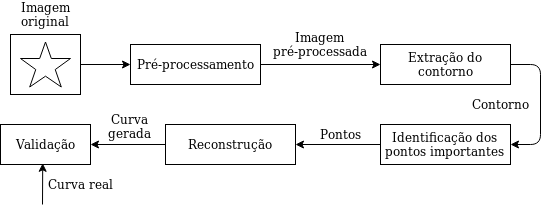
\includegraphics[width=0.9\linewidth]{imagens/diagrama.png}
	\caption{Block diagram of development.}
	\label{fig:diagrama}
	\end{figure}
	The preprocessing aims to eliminate noise on the contour, allowing the extraction of a curvature that better fits it. The identification of important points is done calculating the discrete curvature of the contour. The curve reconstruction is based on a method describe by Sorkine \cite{sorkine} using a few points (called anchor) and connectivity information, by a discretization of the Laplace-Beltrami operator.
	
	
	\section*{\hfil Results}
	
	Some results were obtained on closed curves in $\mathbb{R}^2$, extracted from images of leafs and human faces. The method was also tested on $\mathbb{R}^3$ curves, open curves and polygonal meshes. The figure \ref{fig:leafs} shows an example from the analysis of a tree leaf.

	\begin{figure}[ht!]
		\centering
		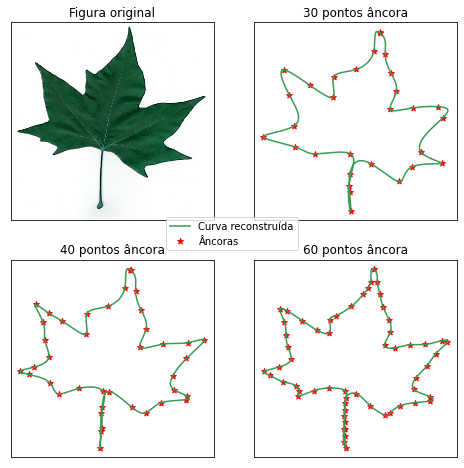
\includegraphics[width=0.9\linewidth]{imagens/leafs.png}
		\caption{Reconstruction of an image of a leaf.}
		\label{fig:leafs}
	\end{figure}
	
	
	\section*{\hfil Conclusions}
	The discrete Laplace-Beltrami operator allows a good reconstruction, given that the anchor points are sufficiently numbered and chosen (for example, using the curvature). However, some details of the original mesh can be lost, as they are not always chosen by the algorithm.
	
	\bibliographystyle{unsrt}
	\renewcommand\refname{\hfil References \hfil}
	\begin{center}
	\begin{thebibliography}{LLL}	
	\bibitem{sorkine}{SORKINE, O. Differential representations for mesh processing. \textit{Computer Graphics Forum}, European Association for Computer Graphics, v. 25, n. 4, p. 789–807, 2006.}
	\end{thebibliography}
	\end{center}
	
	\section*{\hfil Support}
	The project is supported by FAPESP (Fundação de Amparo à Pesquisa do Estado de São Paulo), nr. 2020/07224-5, which is part of the FAPESP Thematic Project nr. 2019/07316-0.
	
	
\end{document}

